\documentclass[10pt,notitlepage,oneside,a4paper]{article}
\usepackage[utf8]{inputenc} 
\usepackage[T1]{fontenc}
\usepackage[spanish]{babel}
\usepackage{datetime} % Personalizar \today
\usepackage{graphicx}
\usepackage{parskip} 
\usepackage{array}
\usepackage{bm} % bold math symbols
\usepackage[a4paper,includeheadfoot,top=1cm,bottom=1cm,left=2cm,right=2cm,head=1.5cm,text=25cm]{geometry} %márgenes
\usepackage{fancyhdr}
\usepackage{fancyvrb}
\usepackage{pstricks}
\usepackage[most]{tcolorbox} % cajas con color de fondo
\usepackage{titlesec}
\usepackage{titletoc}
\usepackage{totpages}
\usepackage{tocloft} % Cambiar aspecto de la tabla de contenidos
\usepackage{siunitx}
\usepackage{booktabs} % Tablas con mejor aspecto
\usepackage{longtable} % tablas que ocupan más de una hoja
\usepackage{enumerate} % http://ctan.org/pkg/enumerate para enumerar con romanos minúsculas
\usepackage{multirow} % http://ctan.org/pkg/multirow
\usepackage{multicol}
\usepackage[hypcap,font=small,labelfont=bf]{caption} % captionof, con hycap usa la parte superior como referencia
\usepackage{capt-of} % Para usar caption fuera de table o figure (flotados)
\usepackage{float} % posicionamiento H para evitar flotar tablas y figuras
\usepackage[draft,inline,nomargin,lang=spanish,author=]{fixme} % notas
\fxsetup{theme=color}
\usepackage[backref,pdfencoding=auto,colorlinks=true,linkcolor=blue]{hyperref}
\usepackage{bookmark} % corrige errores con appendix e hyperref

\graphicspath{{./imagenes/}{./docs/imagenes/}}
\renewcommand{\familydefault}{phv} %phv - Helvética para fuente por defecto
\renewcommand{\headrulewidth}{0pt} % Sin línea superior en encabezado
\addto\captionsspanish{\def\tablename{Tabla}} %% Para renombrar cuadros a tablas

\definecolor{block-gray}{gray}{0.95}
\newtcolorbox{myquote}{colback=block-gray,grow to right by=-10mm,grow to left by=-10mm,
boxrule=0pt,boxsep=0pt,breakable}

% Indentados de ToC
\cftsetindents{section}{0em}{5.5em}
\cftsetindents{subsection}{2em}{3.5em}

\setcounter{secnumdepth}{3} %% Hasta que nivel se numeran las secciones
\setcounter{tocdepth}{3} %% Cuantos niveles aparecen en el indice

%% FORMATOS PÁGINA ************************************************************
%% ------------ PÁGINA INICIAL
\makeatletter
\def\ps@portada{%
\def\@oddhead{
\includegraphics[height=1.17cm]{mfom}\hfill 
\includegraphics[height=1.17cm]{ietcc}~
\includegraphics[height=1.17cm]{csic2}}
\def\@evenhead{
\includegraphics[height=1.17cm]{mfom}\hfill 
\includegraphics[height=1.17cm]{ietcc}~
\includegraphics[height=1.17cm]{csic2}}
%\let\@oddhead\@empty%
%\let\@evenhead\@empty%
\def\@oddfoot{\scriptsize\parbox[b]{4cm}{Versión \version ~/ \fecha \\Página~\textbf{\thepage}~de~ \textbf{\ref*{TotPages}}}\hfill
\rule{.2pt}{1.0cm}\quad \parbox[b]{3.5cm}{C/ SERRANO GALVACHE 4\\28033
MADRID ESPAÑA\\TEL: 91 302 04 40\\FAX: 91 302 07 00}
}%
\def\@evenfoot{\scriptsize\parbox[b]{4cm}{Versión \version ~/ \fecha \\Página~\textbf{\thepage}~de~ \textbf{\ref*{TotPages}}}\hfill
\rule{.2pt}{1.0cm}\quad \parbox[b]{3.5cm}{C/ SERRANO GALVACHE 4\\28033
MADRID ESPAÑA\\TEL: 91 302 04 40\\FAX: 91 302 07 00}
}%
}
\makeatother
%% ------------ PÁGINA plain (para ToC)
\fancypagestyle{plain}{%
\fancyhf{} % clear all header and footer fields
\fancyhead[L]{
\includegraphics[height=1.17cm]{mfom}}
\fancyhead[R]{\hfill 
\includegraphics[height=1.17cm]{ietcc}~
\includegraphics[height=1.17cm]{csic2}\\
\scshape \tiny Instituto de Ciencias de la Construcción Eduardo Torroja}
\fancyfoot[L]{\scriptsize\parbox[b]{4cm}{Versión \version ~/ \fecha \\Página~\textbf{\thepage}~de~ \textbf{\ref*{TotPages}}}}
\renewcommand{\headrulewidth}{0pt}
\renewcommand{\footrulewidth}{0pt}
}
%% ------------ PÁGINA TIPO
\pagestyle{fancy}
\fancyhf{}
\lhead{
\includegraphics[height=1.17cm]{mfom}}
\rhead{\hfill 
\includegraphics[height=1.17cm]{ietcc}~
\includegraphics[height=1.17cm]{csic2}\\
\scshape \tiny Instituto de Ciencias de la Construcción Eduardo Torroja
}
\lfoot{\scriptsize \parbox[b]{4cm}{Versión \version ~/ \fecha \\Página~\textbf{\thepage}~de~ \textbf{\ref*{TotPages}}}}
%% FIN FORMATOS ***************************************************************

%% DATOS DEL INFORME **********************************************************
\newcommand{\titulo}{Manual de usuario del programa \texttt{epbdcalc}}
\newcommand{\subtitulo}{Cálculo de la eficiencia energética según la norma ISO/DIS 52000-1:2015}
\newcommand{\titulocorto}{\titulo} % Título para encabezados
%\newcommand{\tipo}{BORRADOR}%{Documento preliminar} % Tipo documento: PRELIMINAR, FINAL, ETC.
\newdateformat{mydate}{\monthname[\THEMONTH] \THEYEAR}
\newcommand{\fecha}{\mydate\today} % Fecha DD/MM/AAAA o \today para hoy
\newcommand{\version}{1.0}
%% FIN DATOS DEL INFORME ******************************************************

\begin{document}

%% PORTADA *****************************************
\thispagestyle{portada}
\null\vspace{5cm}
%\null\vfill % Usamos párrafo nulo ya que vfill/vspace funciona entre párrafos
\begin{center}
{\Large \bfseries \titulo}
\vskip 0pt\vspace{0.5cm}{\large \subtitulo}
%\vskip 0pt\vspace{0.5cm}{\large \tipo}
\end{center}
%\null\vfill

%% NOTA *****************************************
\null\vfill
%%% AUTORES -----------------------------------------
\begin{center} \footnotesize

\fbox{\parbox{.75\textwidth}{
\textbf{\copyright ~ 2015 Ministerio de Fomento}\\
\textbf{\phantom{\copyright ~ 2015 }Instituto de Ciencias de la Construcción Eduardo Torroja (IETcc-CSIC)}\\[5pt]
\textbf{Autores}:\\[5pt]
\-\qquad Rafael Villar Burke \href{mailto:pachi@ietcc.csic.es}{<pachi@ietcc.csic.es>}\\
\-\qquad Daniel Jiménez González \href{mailto:danielj@ietcc.csic.es}{<danielj@ietcc.csic.es>}
}} %% Nombre de los autores del informe

%\fbox{\parbox{.6\textwidth}{
%\textbf{Nota:}\\[5pt]
%El presente borrador es para uso exclusivo de la persona o entidad a la que está
%dirigido, el receptor le concederá con carácter general la calificación de
%información reservada y restringida.
%
%Los contenidos o ideas recogidas en el mismo pertenecen a sus autores. Se trata
%de un documento preliminar de trabajo y no tiene carácter reglamentario. Los
%autores no se hacen responsables del uso indebido del mismo.
%}} %% Nota

\end{center}
\vskip 0pt\vspace{1.5cm}
\clearpage

\newpage
%% INDICE %%%%%%%%%%%%%%
\tableofcontents
\clearpage

%% DOCUMENTO %%%%%%%%%%%%%%
\newpage
\section{Introducción}

La norma \textit{ISO/DIS 52000-1:2015 (anterior prEN~15603:2014)} de \textit{Eficiencia energética de los edificios. Consumo global de energía y definición de las evaluaciones energéticas} establece la metodología para el cálculo la eficiencia energética dentro del alcance de la \textit{Directiva 2010/31/UE} relativa a la\textit{eficiencia energética de los edificios} (\textit{EPDB}). Para facilitar la comprensión e interpretación de la norma, se desarrolla el informe técnico \textit{FprCEN-TR\_15615: ''Energy Performance of buildings - Acompanying Technical Report on draft Overarching standard EPB (prEN 15063)''} y unas hojas de cálculo asociadas.

Este manual documenta el programa \texttt{epbdcalc}, elaborado por el \textit{Instituto de Ciencias de la Construcción Eduardo Torroja (IETcc-CSIC)} en el marco del convenio vigente con el \textit{Ministerio de Fomento}, que implementa la metodología de cálculo descrita en el último borrador disponible de la norma \textit{ISO/DIS 52000-1:2015 (anterior prEN~15603:2014)}. El programa se ha desarrollado como parte del proceso de trasposición de la directiva a la legislación nacional española y con el objetivo de facilitar la adaptación de las herramientas de evaluación de la eficiencia energética.

El manual describe la interfaz de usuario del programa \textit{epbdcalc} y el formato de los archivos de entrada, que incluyen los valores de producción y consumo energético del edificio.
El programa calcula la energía importada de las redes de abastecimiento, el porcentaje de energía exportada que se considera en la evaluación de la eficiencia energética del edificio. Para todo ello, tiene en cuenta los factores de paso normativos de los distintos vectores energéticos y los factores de resuministro ($k_{rdel}$) y exportación ($k_{exp}$).

\begin{myquote}\footnotesize
    The still-in-progress CEN/ISO standard \textit{ISO/DIS 5200-1:2015 (former prEN~15603:2014)}, on \textit{Energy Efficiency of Buildings. Overarching standard EPB}, sets a framework for the assessment of the energy performance of buildings that is consistent with the \textit{EPB Directive recast (2010/31/UE)} on the \textit{energy efficiency of buildings}. To ease the understanding and interpretation of this standard, the \textit{FprCEN-TR\_15615: ''Energy Performance of buildings - Acompanying Technical Report on draft Overarching standard EPB (prEN 15603)''} has been developed, along with a set of examples in spreadsheet form.

This manual documents the \texttt{epbdcalc} application which has been developed under the current agreement by the \textit{Instituto de Ciencias de la Construcción Eduardo Torroja (IETcc-CSIC)} and the spanish \textit{Ministerio de Fomento} and implements the calculation methodology in the current draft of the standard. It has been developed as part of the transposition process of the EPBD into the spanish legislation and to ease the adaptation of the existing energy evaluation tools.

The manual describes the user interface of the\textit{epbdcalc} application and it input and output formats, including the building energy use and generation.
The application evaluates both the delivered and exported energy according to the evaluation framework. It takes into consideration the different energy factors for each energy carrier as well as the redeliverd energy factor ($k_{rdel}$) and the exported energy factor ($k_{exp}$).
\end{myquote}

\section{Uso del programa}
\label{sec:usoprograma}

\subsection{Interfaz de usuario}

La interacción con el programa se produce a través de la línea de comandos (señalada con \$ en este texto), realizando una llamada al archivo ejecutable \texttt{epbdcalc} (o \texttt{epbdcalc.exe}) en la que se debe indicar la ruta al archivo con los datos energéticos del edificio\footnote{Estos datos se obtienen a partir del proceso de los resultados de un programa de evaluación de la eficiencia energética}, del siguiente modo:

\begin{Verbatim}[fontsize=\small]
	$ epbdcalc ./directorio/datos_entrada.csv
\end{Verbatim}


La ejecución del programa realiza el procesado del archivo de entrada de datos (\texttt{datos\_entrada.csv} en el ejemplo) y resulta en la generación de un archivo de igual nombre con el sufijo \texttt{\_salida}, almacenado en el directorio del archivo de datos, con el resultado del cálculo del balance de energía primaria.

La invocación del programa sin un archivo de datos de entrada o usando las opciones \texttt{-h} o \texttt{--help}:

\begin{Verbatim}[fontsize=\small]
	$ epbdcalc --h
\end{Verbatim}


 muestra la ayuda de uso:

\begin{Verbatim}[fontsize=\small]
    usage: epbdcalc.py [-h] [-f [FPFILE]] [--krdel [KRDEL]] [--kexp [KEXP]] vecfile

	versión: 1.0
	(c) 2015-2016 Ministerio de Fomento
	    2015-2016 Instituto de Ciencias de la Construcción Eduardo Torroja (IETcc-CSIC)
	Autores: Daniel Jiménez González <danielj@ietcc.csic.es>
	         Rafael Villar Burke <pachi@ietcc.csic.es>

    Cálculo de la eficiencia energética según ISO/DIS 52000-1:2015 y CTE DB-HE

    positional arguments:
      vecfile               archivo de datos de los vectores energéticos
    optional arguments:
      -h, --help            show this help message and exit
      -f [FPFILE], --factores [FPFILE]
                            archivo de definición de los factores de paso
      --krdel [KRDEL]       factor de resuministro (k_rdel)
      --kexp [KEXP]         factor de exportacion (k_exp)
      -o [OUTPUTFILE], --outfile [OUTPUTFILE]
                        archivo de salida de resultados
\end{Verbatim}


El programa está concebido para calcular la eficiencia energética con los factores de paso y los parámetros de resuministro y exportación normativos, aunque, mediante distintas opciones del programa es posible realizar los cálculos con otros valores.

Por ejemplo, los archivos de prueba que se distribuyen con el programa usan un archivo de factores de paso del siguiente modo:

\begin{Verbatim}[fontsize=\small]
	$ epbdcalc ../examples/ejemplo1base.csv -f ../examples/factores_paso_test.csv 
\end{Verbatim}

Igualmente, se podría fijar el factor de exportación ($k_{exp}$) así:

\begin{Verbatim}[fontsize=\small]
	$ epbdcalc ../examples/ejemplo1xPV.csv -f ../examples/factores_paso_test.csv --kexp=0.0
\end{Verbatim}

\subsection{Entrada de datos}

El archivo de datos de entrada proporciona la información de origen y uso de la energía en cada paso de calculo. Para ello usa el formato de \textit{valores separados por comas}\footnote{El formato está documentado en el estándar RFC 4180 (\url{https://tools.ietf.org/html/rfc4180}). Consiste en un archivo de texto que describe una tabla de datos, con una línea por cada fila (registro) y donde los valores de las columnas están separados por comas y usan como separador decimal el punto. Opcionalmente, se puede incluir una línea inicial que da nombre a las columnas} con la siguiente estructura de los registros (filas) de datos, que se muestra de forma esquemática en la \autoref{fig:estructuraVectores}:

\begin{itemize}
\item campo \texttt{vector}, de nombre del vector energético;
\item campo \texttt{tipo}, tipo de vector energético (producción o consumo);
\item campo \texttt{origenouso}, de identificación de origen o destino de la energía transferida;
\item campos \texttt{valor}, con un dato para cada paso de tiempo.
\end{itemize}

\begin{figure}[H]
\centering
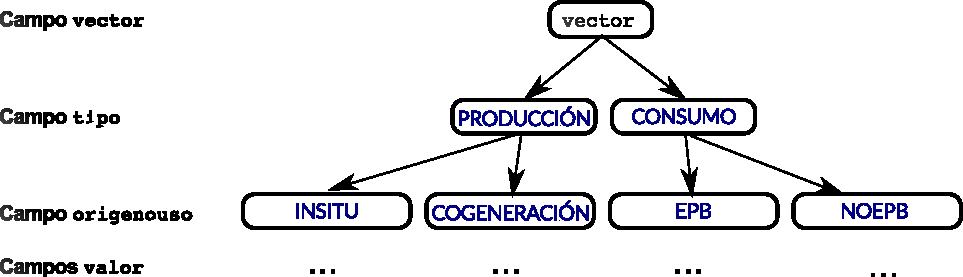
\includegraphics[width=15cm]{esquemavectores}
\caption{Esquema de campos de un registro del archivo \texttt{CSV} de entrada.}
\label{fig:estructuraVectores}
\end{figure}

A continuación se muestra un ejemplo de un conjunto de registros:

\begin{Verbatim}[fontsize=\small,frame=single]
    vector,tipo,origenouso
    ELECTRICIDAD,CONSUMO,EPB,200.10,160.00,100.32,90.56,50.11,60.00,80.00,70,50,80,120,160
    ELECTRICIDAD,CONSUMO,NEPB,30,30,30,30,30,30,30,30,30,30,30,30
    ELECTRICIDAD,PRODUCCION,INSITU,44,55,77,110,187,209,220,198,176,132,88,55
\end{Verbatim}

Los valores admitidos en cada uno de los campos del registro se especifican en los siguientes apartados.

\subsubsection{Campo \texttt{vector}}

Las cadenas de texto admitidas para identificar los vectores energéticos en el campo \texttt{vector} son las siguientes:

\begin{multicols}{3}
\begin{itemize}
\item \texttt{ELECTRICIDAD}
\item \texttt{ELECTRICIDADCANARIAS}
\item \texttt{ELECTRICIDADBALEARES}
\item \texttt{ELECTRICIDADCEUTAMELILLA}
\item \texttt{GASOLEO}
\item \texttt{FUELOIL}
\item \texttt{GLP}
\item \texttt{GASNATURAL}
\item \texttt{CARBON}
\item \texttt{BIOMASA}
\item \texttt{BIOMASADENSIFICADA}
\item \texttt{BIOCARBURANTE}
\item \texttt{MEDIOAMBIENTE}
\item \texttt{COGENERACION}
\end{itemize}
\end{multicols}

\subsubsection{Campo \texttt{tipo}}

El campo \texttt{tipo} puede únicamente contener las cadenas:

\begin{itemize}
\item \texttt{PRODUCCION}
\item \texttt{CONSUMO}
\end{itemize}

Con las siguientes particularidades:

\begin{itemize}
\item Se entiende que todos los suministros pertenecen a la categoría de producción;
\item los suministros de la red no tienen que ser especificados cuando este sea único por vector energético.
\end{itemize}

\subsubsection{Campo \texttt{origenouso}}

El campo \texttt{origenouso} contiene información sobre el origen o destino de la energía.

Para registros en los que el campo \texttt{tipo} sea igual a \texttt{PRODUCCION}, los valores admitidos para cada vector energético y que definen el origen de la producción, son los definidos en la \autoref{tab:fuentesPermitidas}. En esta tabla se observa cómo se considera la producción de vectores energéticos distintos a los de la red únicamente en el caso de la electricidad o de procesos que extraen energía del medio ambiente. Igualmente, se diferencia la electricidad producida \textit{in situ} mediante cogeneración del resto de producción eléctrica \textit{in situ}.

\begin{table}[H]
\centering
\small
\caption{Valores admitidos para el campo \texttt{origenouso} para la producción de energía}\label{tab:fuentesPermitidas}
\begin{tabular}{ll}
    \toprule
    \textbf{Vector definido en el campo \texttt{vector}} & \textbf{Valores admitidos del campo \texttt{origenouso}}\\
    \midrule
    \texttt{ELECTRICIDAD}             & \texttt{INSITU}, \texttt{COGENERACION}\\
    \texttt{ELECTRICIDADCANARIAS}     & \texttt{INSITU}, \texttt{COGENERACION}\\
    \texttt{ELECTRICIDADBALEARES}     & \texttt{INSITU}, \texttt{COGENERACION}\\
    \texttt{ELECTRICIDADCEUTAMELILLA} & \texttt{INSITU}, \texttt{COGENERACION}\\
    \texttt{MEDIOAMBIENTE}            & \texttt{INSITU}\\
    \bottomrule
\end{tabular}
\end{table}

Para registros en los que el campo \texttt{tipo} sea igual a \texttt{CONSUMO}, es necesario especificar si la energía se destina a usos evaluados en la eficiencia energética (usos EPB) o usos no evaluados (usos no EPB), de modo que los valores permitidos son los siguientes:

\begin{itemize}
\item \texttt{EPB}
\item \texttt{NEPB}
\end{itemize}

\subsubsection{Campos \texttt{valor}}

Estos campos contienen los valores numéricos de consumo o producción para cada paso de tiempo, usando el punto como separador decimal (se recomienda el uso de dos decimales).

En el caso de que en un archivo aparezcan varios registros con idénticos valores en los campos \texttt{vector}, \texttt{tipo} y \texttt{origenouso}, el programa sumará los datos de los campos \texttt{valor} en cada paso de tiempo y trabajará como si se hubiese definido un único registro con la suma de los datos. Esto permite dejar al programa la tarea de agregación de valores y puede resultar últi, por ejemplo, para definir las producciones electricas de varios sistemas fotovoltaicos.

Todos los registros deben emplear número igual de pasos de tiempo, o el programa emitirá un error.

\subsection{Salida de resultados}

La norma \textit{ISO/DIS 52000-1:2015} establece como indicadores de la eficiencia energética de los edificios el \textit{consumo total de energía primaria} (\texttt{$EP_{tot}$}) y el \textit{porcentaje de energía primaria renovable del consumo total de energía} (\texttt{$RER$}).

El programa ofrece, además de dichos indicadores (para los pasos A+B y A), la descomposición consumo total de energía primaria en su parte renovable (\texttt{$EP_{ren}$}) y no renovable (\texttt{$EP_{nren}$}), como se muestra en la \autoref{tab:indicadoresFinales}.

\begin{table}[H]
\centering
\small
\caption{Indicadores de la eficiencia energética obtenidos con el programa}\label{tab:indicadoresFinales}
\begin{tabular}{ll}
    \toprule
    \textbf{Indicador} & \textbf{Descripción}\\
    \midrule
    \texttt{EPren}  & Parte renovable de la energía primaria total\\
    \texttt{EPnren} & Parte no renovable de la energía primaria total\\
    \texttt{EPtot}  & Consumo total de energía primaria\\
    \texttt{RER}    & Fracción de energía primara renovable en el consumo total\\
    \bottomrule
\end{tabular}
\end{table}

Esta salida se realiza a través de la salida estándar, pudiendo indicar mediante la opción \texttt{-o} o \texttt{--outfile} que se almacene en un archivo, tal como se describe en el la sección \autoref{sec:usoprograma}, de \nameref{sec:usoprograma}. A continuación se muestra un ejemplo de la salida generada:

\VerbatimInput[fontsize=\small, frame=lines, rulecolor=\color{gray}]{../pyepbd/examples/ejemplo1base_salida.csv}

\clearpage
\newpage

%%% ANEXOS *******************************************************************************

\setcounter{section}{0} % resetear contador de secciones
\renewcommand\thesection{Anexo~\Roman{section}}
\renewcommand\theHsection{Anexo~\Roman{section}}
\renewcommand\thesubsection{\Roman{section}.\arabic{subsection}}
\renewcommand\theHsubsection{\Roman{section}.\arabic{subsection}}
\renewcommand{\thefigure}{\Roman{section}.\arabic{figure}}
\renewcommand{\theHfigure}{\Roman{section}.\arabic{figure}}
\renewcommand{\thetable}{\Roman{section}.\arabic{table}}
\renewcommand{\theHtable}{\Roman{section}.\arabic{table}}

\section{Ejemplos}
\label{sec:anexoejemplos}
\setcounter{figure}{0} % resetear contador por sección
\setcounter{table}{0} % resetear contador por sección

Para ilustrar el funcionamiento del programa se han implementado los ejemplos del anejo K del documento técnico \textit{FprCEN-TR\_15615} que acompaña a la norma.

Estos test se han realizado con los mismo factores de paso de ejemplo que contiene la norma, por lo que para reproducir los resultados es necesario usar esos factores. En la llamada al programa se incluye como parámetro el nombre del archivo que contiene esos factores de paso.

\subsection{Ejemplo 1: Sistema totalmente eléctrico}
El ejemplo 1 es un sistema totalmente eléctrico en el que contemplan distintas variantes en función de la cantidad de energía fotovoltaica que se produce.


\subsubsection{Caso base}
 
En el caso base todos los sistemas del edificio funcionan con un único vector energético, la electricidad, y no hay aportes de otro tipo. Esto excluye a las bombas de calor, puesto que en ese caso se consideraría que el medioambiente aporta otro vector energético. El consumo en servicios EPB es de 100 kWh y no se considera consumo para otros usos.

El archivo de definición del caso sería (\texttt{ejemplo1base.csv}):

\VerbatimInput[fontsize=\small, frame=lines, rulecolor=\color{gray}]{../pyepbd/examples/ejemplo1base.csv}

La llamada al programa se realizaría así:

\begin{Verbatim}[fontsize=\small]
    $ epbdcalc ejemplo1base.csv -f factores_paso_test.csv
\end{Verbatim}

El archivo de salida (\texttt{ejemplo1base\_salida.csv}):

\VerbatimInput[fontsize=\small, frame=lines, rulecolor=\color{gray}]{../pyepbd/examples/ejemplo1base_salida.csv}

\subsubsection{Aporte de energía fotovoltaica}

Una variante del anterior supone la introducción de energía fotovoltaica por un valor de la mitad de lo consumido en EPB, de 50 kWh. De manera que se añade un concepto que refleje este aporte (\textit{ejemplo1PV.csv}):

\VerbatimInput[fontsize=\small, frame=lines, rulecolor=\color{gray}]{../pyepbd/examples/ejemplo1PV.csv}

La llamada al programa se realizaría así:

\begin{Verbatim}[fontsize=\small]
    $ epbdcalc ejemplo1PV.csv -f factores_paso_test.csv
\end{Verbatim}

Que daría como resultado (\textit{ejemplo1PV\_salida.csv}):

\VerbatimInput[fontsize=\small, frame=lines, rulecolor=\color{gray}]{../pyepbd/examples/ejemplo1PV_salida.csv}

\subsubsection{Exceso de energía fotovoltaica}

En esta ocasión el sistema fotovoltaico produce más energía de la que se demanda para cubrir los servicios EPB. Este hecho se refleja en la entrada de datos \texttt{ejemplo1xPV.csv}):

\VerbatimInput[fontsize=\small, frame=lines, rulecolor=\color{gray}]{../pyepbd/examples/ejemplo1xPV.csv}

La llamada al programa se realizaría así:

\begin{Verbatim}[fontsize=\small]
    $ epbdcalc ejemplo1xPV.csv -f factores_paso_test.csv
\end{Verbatim}
%$

Los valores de salida son \texttt{ejemplo1xPV.csv}:

\VerbatimInput[fontsize=\small, frame=lines, rulecolor=\color{gray}]{../pyepbd/examples/ejemplo1xPV_salida.csv}

\subsection{Ejemplo 2: Sistema de gas natural con apoyo eléctrico}
En el ejemplo 2 la demanda energética es cubierta con una caldera que consume 190 kWh, existiendo un consumo eléctrico menor de apoyo de 20 kWh. Además existe una instalación fotovoltaica que aporta 40 kWh anuales. Todo ello queda recogido en el fichero de datos \texttt{ejemplo2PVgas.csv}:

\VerbatimInput[fontsize=\small, frame=lines, rulecolor=\color{gray}]{../pyepbd/examples/ejemplo2PVgas.csv}

La llamada al programa se realizaría así:

\begin{Verbatim}[fontsize=\small]
    $ epbdcalc ejemplo2PVgas.csv -f factores_paso_test.csv
\end{Verbatim}

El resultado es (\texttt{ejemplo2PVgas\_salida.csv}):

\VerbatimInput[fontsize=\small, frame=lines, rulecolor=\color{gray}]{../pyepbd/examples/ejemplo2PVgas_salida.csv}

\subsection{Ejemplo 3: Sistema de bomba de calor con apoyo fotovoltaico.}
El ejemplo 3 recoge el caso de un sistema con bomba de calor que cubre toda la demanda de EPB. Esta bomba de calor eléctrica consume 59 kWh, de los cuales 40 son de origen fotovoltaico. Esa energía se usa para bombear 131 kWh del medio ambiente. El archivo de definición \texttt{ejemplo3PVBdC.csv}:

\VerbatimInput[fontsize=\small, frame=lines, rulecolor=\color{gray}]{../pyepbd/examples/ejemplo3PVBdC.csv}

La llamada al programa se realizaría así:

\begin{Verbatim}[fontsize=\small]
    $ epbdcalc ejemplo3PVBdC.csv -f factores_paso_test.csv
\end{Verbatim}

Los valores de salida son (\texttt{ejemplo3PVBdC\_salida.csv}):

\VerbatimInput[fontsize=\small, frame=lines, rulecolor=\color{gray}]{../pyepbd/examples/ejemplo3PVBdC_salida.csv}

\subsection{Ejemplo 4: Caldera y sistema de cogeneración con combustible fósil.}
En el ejemplo 4 hay presente una caldera de gas natural que consume 100 kWh y una máquina de cogeneración que consume 158 kWh, también de gas natural. Como resultado de la cogeneración se generan 48 kWh de electricidad de los cuales 28 son exportados a la red. La entrada de datos sería la recogida en el archivo \texttt{ejemplo4cgnfosil.csv}:

\VerbatimInput[fontsize=\small, frame=lines, rulecolor=\color{gray}]{../pyepbd/examples/ejemplo4cgnfosil.csv}

La llamada al programa se realizaría así:

\begin{Verbatim}[fontsize=\small]
    $ epbdcalc ejemplo4cgnfosil.csv -f factores_paso_test.csv
\end{Verbatim}

El resultado es (\texttt{ejemplo4cgnfosil\_salida.csv}):

\VerbatimInput[fontsize=\small, frame=lines, rulecolor=\color{gray}]{../pyepbd/examples/ejemplo4cgnfosil_salida.csv}

\subsection{Ejemplo 5: Caldera y sistema de cogeneración con combustible renovable.}
Este ejemplo 5 es idéntico al anterior con la salvedad de que los 158 kWh que consume el sistema de cogeneración provienen de fuentes renovables (\texttt{ejemplo5cgnbiogas.csv}):

\VerbatimInput[fontsize=\small, frame=lines, rulecolor=\color{gray}]{../pyepbd/examples/ejemplo5cgnbiogas.csv}

La llamada al programa se realizaría así:

\begin{Verbatim}[fontsize=\small]
    $ epbdcalc ejemplo5cgnbiogas.csv -f factores_paso_test.csv
\end{Verbatim}

La salida es \texttt{ejemplo5cgnbiogas\_salida.csv}:

\VerbatimInput[fontsize=\small, frame=lines, rulecolor=\color{gray}]{../pyepbd/examples/ejemplo5cgnbiogas_salida.csv}


\subsection{Ejemplo 6: Calculo con varios pasos y valores para no EPB}
En el apartado K.3 del informe técnico se comenta mediante variaciones de un caso como se trata la energía exportada temporalmente y resuministrada posteriormente. El paso de cálculo es mensual, ya que con un paso anual no tendría sentido la idea de resuministro.

Además sí se consideran una serie de consumos energéticos para servicios que no van a incluirse dentro de la eficiencia energética del edificio, pero que hay que tenerlos en cuenta en el balance como energía exportada. 

El sistema se tan simple como el del ejemplo 1, con la variante de la existencia de un sistema fotovoltaico que aporta una parte del consumo eléctrico. Los valores de entrada corresponden a la tabla K.1 del citado informe (\texttt{ejemplo6K3.csv}):

\VerbatimInput[fontsize=\small, frame=lines, rulecolor=\color{gray}]{../pyepbd/examples/ejemplo6K3.csv}

La llamada al programa se realizaría así:

\begin{Verbatim}[fontsize=\small]
    $ epbdcalc ejemplo6K3.csv -f factores_paso_test.csv
\end{Verbatim}

Los indicadores de eficiencia energética son \texttt{ejemplo6K3\_salida.csv}:

\VerbatimInput[fontsize=\small, frame=lines, rulecolor=\color{gray}]{../pyepbd/examples/ejemplo6K3_salida.csv}

\end{document}
